At MEDAPP, a sample of strontium-90 is used mainly as a $\beta^-$ check source. It is chosen because the radiation spectrum is comparable to the MEDAPP spectrum and can produce comparable results when it irradiates an ionization chamber. The goal of this chapter is to model the $\beta^-$ check source in MCNP to run a simulation on the PTW magnesium chamber TM33053 to study the effect of the corrosion layer.

As the strontium-90 decays it forms \ce{^{39}_{38}Y} and emits a $\beta ^-$ particle of 0.546 \unit{\mega\electronvolt} \cite{modernlabExperiments} and this \ce{^{90}_{39}Y}, in turn, decays into  \ce{^{90}_{40}Zr} emitting also a $\beta ^-$ particle of 2.274 \unit{\mega\electronvolt} \cite{modernlabExperiments} according to the scheme:

\begin{figure}[!h]
    \centering
    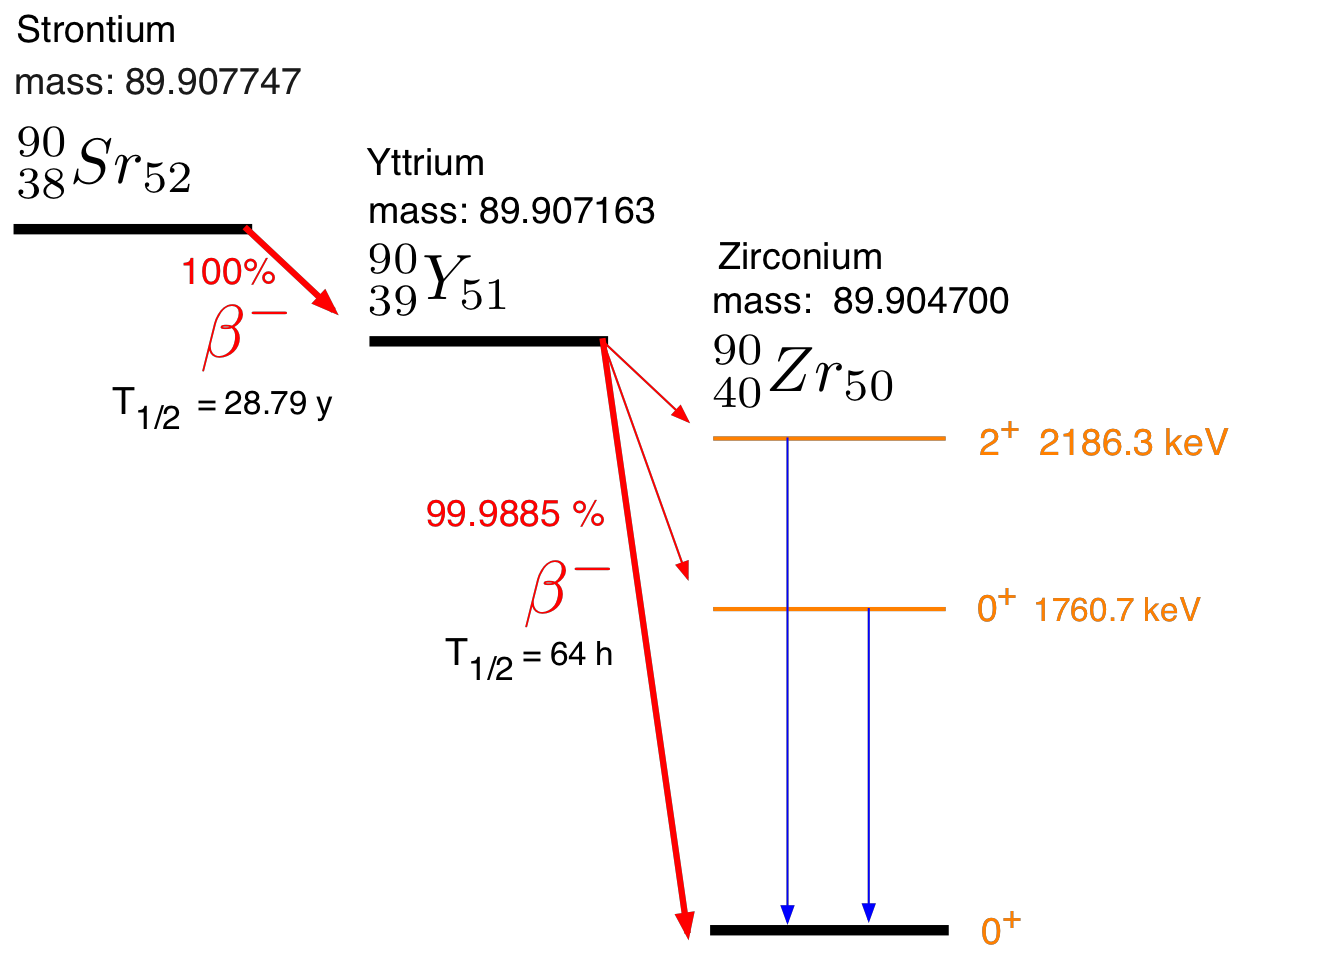
\includegraphics[scale = 0.4]{Master Thesis Manuel Galdon/figures/Sr90_decay.png}
    \caption{Decay scheme of Sr-90, masses and half lives of Sr-90 and daughter nuclei \cite{modernlabExperiments}.}
    \label{fig:Sr90_decay}
\end{figure}


\ce{^{90}{}Sr} primarily emits beta particles during its decay process, making it an important source for various applications, including ionization cameras. The source can also undergo gamma emission due to the two meta-states names as $2^+$ and $0^+$ corresponding to 2186.3 \unit{\kilo\electronvolt} and 1760.7 \unit{\kilo\electronvolt}, respectively. The decay spectrum and the absolute decay probabilities have been consulted and taken from the \emph{Nuclear Data Section} of the \emph{International Atomic Energy Agency} \cite{intlAtomicEnergy}. 

In MCNP, the source is modelled as a continuous source due to the $\beta^-$ particles emission. This implies that the energy is distributed in a non-discrete manner between the emitted electron and the residual nucleus. Consequently, different beta decays can produce electrons at different energies within a specific range. The isotropic strontium source is placed in a designated cell, which is in contact with the air and brass, and it emits $\beta^-$ particles that generates continuous \textit{bremsstrahlung} radiation in all directions. 

An accurate geometrical arrangement  of the source has been performed conform to the sketch of the \emph{Radioaktive Kontrollvorrichtung 39 Typ 8921 für PTW-Dosimeter} \cite{kontrollvorrichtung} issued by PTW. Both the sketch and the simulated geometry of the source are compared in Figure \ref{fig:PTW sketch and simulation}

\begin{figure}[!h]
\centering
\begin{subfigure}{0.4\textwidth}
    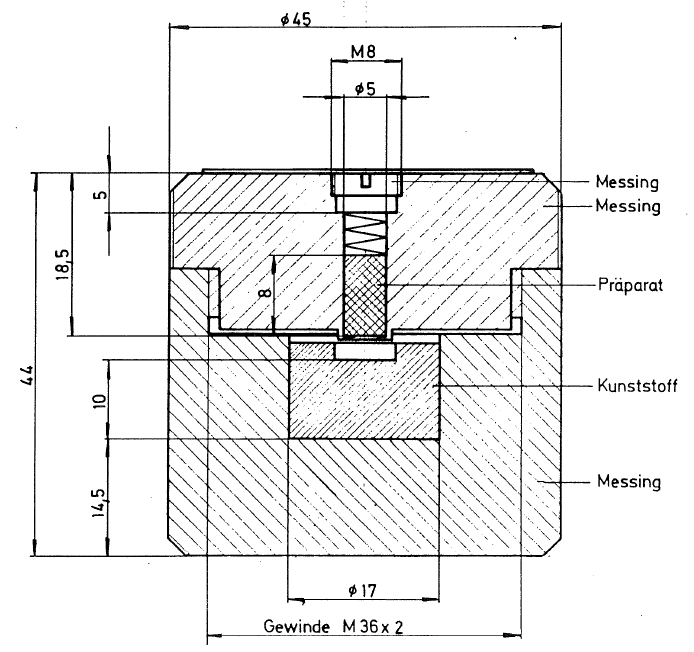
\includegraphics[scale = 0.25]{Master Thesis Manuel Galdon/figures/Sr90-sketch.png} 
    %\caption{Sketch of the \ce{^{90}{}Sr} source of PTW \cite{kontrollvorrichtung}}
        %\label{fig:sr-90_sketch}
\end{subfigure}
\hfill
\begin{subfigure}{0.4\textwidth}
    %\captionsetup{margin={0pt, 45pt}}
    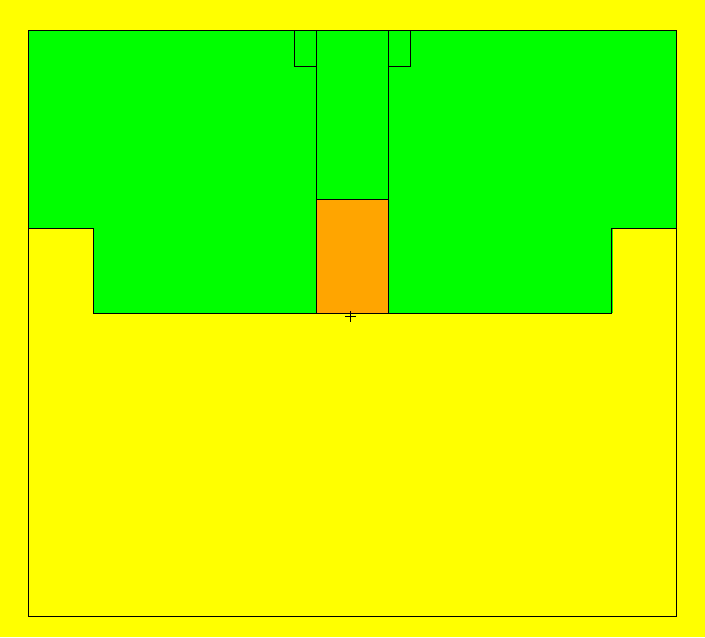
\includegraphics[scale = 0.25]{Master Thesis Manuel Galdon/figures/sr-90.PNG}
    %\caption{Simulation of \ce{^{90}{}Sr} source}
     %   \label{fig:sr-90 Simulation}
\end{subfigure}
        
    \caption{Sketch (left) and simulation (right) of the \ce{^{90}{}Sr} source.}
\label{fig:PTW sketch and simulation}
\end{figure}

The materials are defined conform with the standard established by the compendium of MNCP \cite{matcomposition}. In the simulated source plotted in Figure \ref{fig:PTW sketch and simulation} (right), the yellow area represents dry air, the green part is composed by brass, and the orange cell is made of Sr-90. In the next table there is exposed a more detailed view of the composition of each material: 

\begin{table}[!h]
\centering

\begin{tabular}{l|c|c|c|c|l}
\cline{2-5}
 & Material                 & Composition & ZAID      & Atom fraction &  \\ \cline{2-5}
 & \multirow{4}{*}{Dry air} & C-12         & 6012.80c  & 0.000124      &  \\ \cline{3-5}
 &                          & N-14         & 7014.80c  & 0.755267      &  \\ \cline{3-5}
 &                          & O-16         & 8016.80c  & 0.231781      &  \\ \cline{3-5}
 &                          & Ar-40        & 18040.80c & 0.012827      &  \\ \cline{2-5}
 & \multirow{5}{*}{Brass}   & Fe           & 26000.84p & 0.000868      &  \\ \cline{3-5}
 &                          & Cu           & 29000.84p & 0.665384      &  \\ \cline{3-5}
 &                          & Zn           & 30000.84p & 0.325699      &  \\ \cline{3-5}
 &                          & Sn           & 50000.84p & 0.002672      &  \\ \cline{3-5}
 &                          & P            & 82000.84p & 0.005377      &  \\ \cline{2-5}
\end{tabular}
\caption{MCNP material composition of the dry air and brass \cite{matcomposition}.}
\label{table:composition of Sr-90 source materals}
\end{table}

As it is noticeable in the last table, the entire \emph{ZAID} is included for a more complete reference to the specific atom according to the listing tables of Los Alamos National Laboratory \cite{ACEDataTables}. The density of the dry air at near the sea level altitude is tabulated as 1.205 \unit{\milli\gram\per\cubic\centi\meter} and for brass, its density is tabulated as 8.07 \unit{\milli\gram\per\cubic\centi\meter}.


